\section{Auswertung}
\label{sec:Auswertung}

\subsection{Untersuchung der Filterkurve}

Zunächst wird die Durchlassfrequenz $\nu$ des Selektivverstärkers bestimmt. Die 
gemessenen Wertepaare von Frequenz $\nu$ und Spannung $U_\text{A}$ sind in 
Tabelle \ref{tab:Messdaten1} aufgeführt. 

\begin{table}
\centering
\caption{Messwerte der Filterkurve des Selektivverstärkers.}
\label{tab:Messdaten1}
\sisetup{table-format=2.1}
\begin{tabular}{c c c c}
\toprule
$\nu \,/\, \si{\kilo\hertz}$ & $U_\text{A} \,/\, \si{\milli\volt}$ & $\nu \,/\, \si{\kilo\hertz}$ & $U_\text{A} \,/\, \si{\milli\volt}$\\
\midrule
20,0 &  0,865 & 34,6 & 35,00\\
21,0 &  0,900 & 34,7 & 43,00\\
22,0 &  0,990 & 34,8 & 55,00\\
23,0 &  1,095 & 34,9 & 72,50\\
24,0 &  1,230 & 35,0 & 93,00\\
25,0 &  1,380 & 35,1 & 96,00\\
26,0 &  1,560 & 35,2 & 78,00\\
27,0 &  1,800 & 35,3 & 59,00\\
28,0 &  2,100 & 35,4 & 46,00\\
29,0 &  2,520 & 35,5 & 37,00\\
30,0 &  3,200 & 35,6 & 31,00\\
31,0 &  4,000 & 35,7 & 26,00\\
32,0 &  5,450 & 35,8 & 23,00\\
33,0 &  8,350 & 35,9 & 20,00\\
34,0 & 16,000 & 36,0 & 18,00\\
34,1 & 17,000 & 36,1 & 16,00\\
34,2 & 19,500 & 37,0 &  9,00\\
34,3 & 22,000 & 38,0 &  6,15\\
34,4 & 25,000 & 39,0 &  4,60\\
34,5 & 29,000 & 10,0 &  3,70\\
\bottomrule
\end{tabular}
\end{table}

Die gemessene Frequenz $\nu$ wird gegen die Spannung $U_\text{A}$ aufgetragen. Das 
Ergebnis ist in Abbildung \ref{fig:plot1} zu finden. 

\begin{figure}
  \centering
  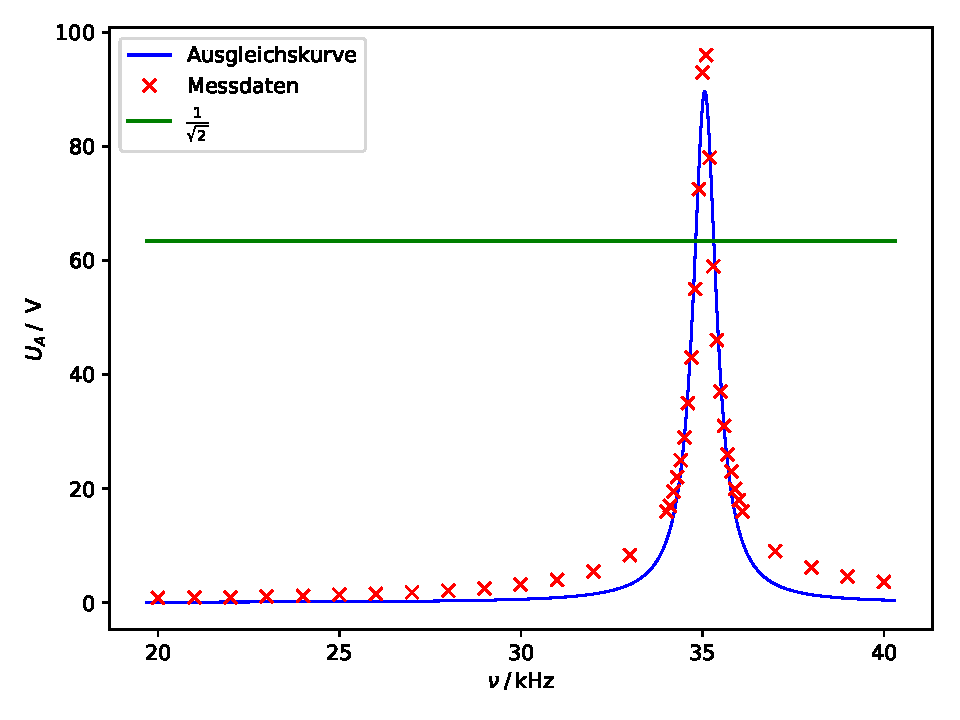
\includegraphics{content/plot1.pdf}
  \caption{Filterkurve des Selektivverstärkers.}
  \label{fig:plot1}
\end{figure}

Mittels Python wird eine Lorentzkurve für eine Ausgleichskurve 
gefittet. Dabei wird die Gleichung 

\begin{equation*}
f(x) = \frac{a}{(x²-x_0^2)²+\gamma²x_0²}
\end{equation*}

für die berechnete Lorentzkurve verwendet. 

Die Durchlassfrequenz lässt sich nun direkt ablesen und ergibt sich zu:

\begin{equation}
x_0 = \nu _\text{A} = \SI{35.065}{\kilo\hertz}.
\end{equation}

Desweiteren wird bei einem Wert von $\frac{1}{\sqrt{2}}$ des Maximalwerts
eine Gerade angelegt. Die Parameter ergeben sich schließlich zu: 

\begin{align*}
a &= \SI{6.6+-0.4e4}{\volt\per\second²},\\
\gamma &= \SI{0.772+-0.031}{}.
\end{align*}

Außerdem werden $\nu_\text{A}$, $\nu_1$ und $\nu_2$ mittels Python zu

\begin{align*}
\nu_1 &= \SI{34.816+-0.014}{\kilo\hertz},\\
\nu_\text{A} &= \SI{35.065+-0.010}{\kilo\hertz},\\
\nu_2 &= \SI{35.313+-0.014}{\kilo\hertz}
\end{align*}

berechnet. Die Güte $Q$ kann nun mit 

\begin{equation*}
Q = \frac{\nu_\text{A}}{\nu_2 - \nu_1}
\end{equation*}

zu 

\begin{equation*}
Q = \num{70.5+-2.8}
\end{equation*}

berechnet werden.
Der Fehler ergibt sich dabei durch eine Fehlerrechnung mittels 
Python.

\subsection{Theoretische Bestimmung des Suszeptibilitäten}

Nach Formel \eqref{eqn:theo} lassen sich die Theoriewerte Seltener 
Erde Verbindungen berechnen. Es werden $\symup{Dy_2O_3}$, $\symup{C_6O_{12}Pr_3}$, 
$\symup{Gd_2O_3}$ und $\symup{Nd_2O_3}$ untersucht. Es wird eine Temperatur von 
$T = \SI{294}{\kelvin}$ angenommen, was etwa Raumtemperatur entspricht.
Der Lande-Faktor $g_J$, sowie $S$, $L$ und $J$ sind in Tabelle \ref{tab:theo} 
aufgeführt.

\begin{table}
\centering
\caption{Theoretische Werte zur Berechnung der Suszeptibilitäten}
\label{tab:theo}
\sisetup{table-format=2.1}
\begin{tabular}{c c c c c}
\toprule
& $\symup{Nd_2O_3}$ & $\symup{Gd_2O_3}$ & $\symup{Dy_2O_3}$ & $\symup{C_6O_{12}Pr_3}$\\
\midrule
4f-Elektronen & 3    & 7   & 9    & 3\\
L             & 6    & 0   & 5    & 5\\
S             & 1,5  & 3,5 & 2,5  & 1\\
J             & 4,5  & 3,5 & 7,5  & 4\\
$g_J$         & 0,97 & 2,0 & 1,41 & 0,8\\
\bottomrule
\end{tabular}
\end{table}

Außerdem ergibt sich $N$ nach

\begin{equation*}
N = \frac{\rho}{M}\cdot N_\text{A}.
\end{equation*}

Dabei ist $N_\text{A} = \SI{6.02214129e23}{1\per\mol}$ [2] die 
Avogadrokonstante, $\rho$ die Dichte des jeweiligen Stoffes und $M$
die molare Masse. Diese Werte sind zusammen mit den berechneten Werten für $N$
in Tabelle \ref{tab:theo2} zu finden. Setzt man diese Werte alle in Gleichung  
\eqref{eqn:theo} ein, so ergeben sich die gesuchten Suszeptibilitäten, die sich ebenfalls in 
Tabelle \ref{tab:theo2} befinden. 

\begin{table}
\centering
\caption{Molare Masse $M$, die Zahl der magnetischen Momente
pro Volumeneinheit $N$ der Seltenen Erden Verbindungen und die berechneten 
Suszeptibilitäten $\chi$.}
\label{tab:theo2}
\sisetup{table-format=2.1}
\begin{tabular}{c c c c c}
\toprule
& $\symup{Nd_2O_3}$ & $\symup{Gd_2O_3}$ & $\symup{Dy_2O_3}$ & $\symup{C_6O_{12}Pr_3}$\\
\midrule
$M/\si{\gram\mol^-1}$            & 168     & 176    & 180    & 346\\
$N \cdot \num{e28}/\si{\meter³}$ & 2,60    & 2,53   & 2,61   & 1,09\\
$\chi$                           & 0,00536 & 0,0142 & 0,0294 & 0,00123\\
\bottomrule
\end{tabular}
\end{table}


\subsection{Experimentelle Bestimmung der Suszeptibilität}

Zunächst muss der Koeffizient Q durch den Querschnitt

\begin{equation}
Q_\text{real} = \frac{m}{\rho \cdot l}
\end{equation}

ersetzt werden. Dieser ergibt sich durch die Länge $l$, die Masse $m$ und 
die Dichte $\rho$ der Probe. Diesen Querschnitt müsste die Probe haben, wenn 
sie aus einem Einkristall bestünde.

\begin{table}
\centering
\caption{$Q_\text{real}$ der verwendeten Stoffe.}
\label{tab:Messdaten2}
\sisetup{table-format=2.1}
\begin{tabular}{c c}
\toprule
Stoff & $Q_\text{real} \,/\, \si{\centi\meter²}$\\
\midrule
$\symup{Gd_2O_3}$ & 0,119\\
$\symup{Dy_2O_3}$ & 0,121\\
$\symup{Nd_2O_3}$ & 0,078\\
$\symup{C_6O_\text{12}Pr_2}$ & 0,079\\
\bottomrule
\end{tabular}
\end{table}

Es wurde mit der Eingangsspannung $U_\text{E} = \SI{0.8}{\volt}$ gemessen. Der 
Spulenquerschnitt ist mit $F = \SI{86.6}{\milli\meter²}$ gegeben. Aus den Messwerten 
können nun die Suszeptibilitäten $\chi$ berechnet werden, nach Bereinigung 
um die Verstärkung $V$. Diese finden sich in Tabelle \ref{tab:Messdaten3}, 
\ref{tab:Messdaten4}, \ref{tab:Messdaten5} und \ref{tab:Messdaten6}.
Dabei bezeichnen $U_\text{m}$ und $R_\text{m}$ die Spannung und Widerstände, 
während die Probe sich in der Spule befindet. $U_\text{0}$ und $R_\text{0}$
sind entsprechend die Werte ohne Probe in der Spule. 

\begin{table}
\centering
\caption{Messwerten und Suszeptibilitäten für $\symup{Dy_2O_3}$}
\label{tab:Messdaten3}
\sisetup{table-format=2.1}
\begin{tabular}{c c c c c}
\toprule
$U_\text{0} \,/\, \si{\milli\volt}$ & $R_\text{0} \,/\, \si{\ohm}$ & $U_\text{m} \,/\, \si{\milli\volt}$& $R_\text{m} \,/\, \si{\ohm}$ & $\chi _\text{exp}$ \\
\midrule
0,135 & 4,375 & 0,385 & 4,232 & 0,0020\\
0,090 & 4,425 & 0,150 & 4,255 & 0,0024\\
0,110 & 4,430 & 0,420 & 4,255 & 0,0025\\ 
\bottomrule
\end{tabular}
\end{table}

\begin{table}
\centering
\caption{Messwerten und Suszeptibilitäten für $\symup{Nd_2O_3}$}
\label{tab:Messdaten4}
\sisetup{table-format=2.1}
\begin{tabular}{c c c c c}
\toprule
$U_\text{0} \,/\, \si{\milli\volt}$ & $R_\text{0} \,/\, \si{\ohm}$ & $U_\text{m} \,/\, \si{\milli\volt}$& $R_\text{m} \,/\, \si{\ohm}$ & $\chi _\text{exp}$ \\
\midrule
0,10 & 4,255 & 0,08 & 4,455 & 0,0045\\
0,08 & 4,455 & 0,08 & 4,565 & 0,0025\\
0,09 & 4,565 & 0,08 & 4,635 & 0,0016\\
\bottomrule
\end{tabular}
\end{table}

\begin{table}
\centering
\caption{Messwerten und Suszeptibilitäten für $\symup{Gd_2O_3}$}
\label{tab:Messdaten5}
\sisetup{table-format=2.1}
\begin{tabular}{c c c c c}
\toprule
$U_\text{m} \,/\, \si{\milli\volt}$ & $R_\text{m} \,/\, \si{\ohm}$ & $U_\text{0} \,/\, \si{\milli\volt}$& $R_\text{0} \,/\, \si{\ohm}$ & $\chi _\text{exp}$ \\
\midrule
0,9 & 4,635 &  0,17 & 4,855 & 0,0032\\
1,0 & 4,500 &  1,90 & 4,860 & 0,0053\\
0,9 & 4,860 & 85,00 & 5,010 & 0,0022\\
\bottomrule
\end{tabular}
\end{table}

\begin{table}
\centering
\caption{Messwerten und Suszeptibilitäten für $\symup{C_6O_{12}Pr_3}$}
\label{tab:Messdaten6}
\sisetup{table-format=2.1}
\begin{tabular}{c c c c c}
\toprule
$U_\text{m} \,/\, \si{\milli\volt}$ & $R_\text{m} \,/\, \si{\ohm}$ & $U_\text{0} \,/\, \si{\milli\volt}$& $R_\text{0} \,/\, \si{\ohm}$ & $\chi _\text{exp}$ \\
\midrule
0,8 & 4,43 &  49 & 4,57 & 0,0031\\
0,9 & 4,57 &  49 & 4,77 & 0,0044\\
0,8 & 4,77 & 1,3 & 4,99 & 0,0049\\
\bottomrule
\end{tabular}
\end{table}

Aus den Suszeptibilitäten können nun die Mittelwerte berechnet werden, 
sodass sich Tabelle \ref{tab:Messdaten7} ergibt. 

\begin{table}
\centering
\caption{Berechnete Suszeptibilitäten.}
\label{tab:Messdaten7}
\sisetup{table-format=2.1}
\begin{tabular}{c c c c c}
\toprule
& $\symup{Gd_2O_3}$ & $\symup{Dy_2O_3}$ & $\symup{Nd_2O_3}$ & $\symup{C_6O_{12}Pr_3}$\\
\midrule
$\chi_\text{theo}$ & 0,0142 & 0,02940 & 0,00536 & 0,00123\\
$\chi_\text{exp}$  & 0,0036 & 0,00230 & 0,00286 & 0,00413\\
\bottomrule
\end{tabular}
\end{table}

Damit ergeben sich die Abweichungen in Tabelle \ref{tab:Messdaten8} vom theoretischem 
Wert. 

\begin{table}
\centering
\caption{Abweichungen zum theoretischem Wert.}
\label{tab:Messdaten8}
\sisetup{table-format=2.1}
\begin{tabular}{c c}
\toprule
& $\frac{\chi_\text{theo}-\chi_\text{exp}}{\chi_\text{theo}}$\\ 
\midrule
$\symup{Dy_2O_3}$       &  $\SI{50.00}{\percent}$\\
$\symup{Nd_2O_3}$       &  $\SI{92.18}{\percent}$\\
$\symup{Gd_2O_3}$       &  $\SI{74.65}{\percent}$\\
$\symup{C_6O_{12}Pr_3}$ & $\SI{234.96}{\percent}$\\
\bottomrule
\end{tabular}
\end{table}

Diese ergeben sich nach 

\begin{equation*}
\nu = \left|\frac{\chi_\text{theo}-\chi_\text{exp}}{\chi_\text{theo}}\right| \cdot 100.
\end{equation*}
